\documentclass[11pt, a4paper]{article}
\usepackage{amsmath}
\usepackage{graphicx}

\title{Versuch 1: Akustik}
\author{Jascha Fricker, Benedict Brouwer}

\begin{document}
    \maketitle

    \section{Abstract}
    In diesem Versuch wird die Schallgeschwindigkeit in verschiedenen elastischen Medien
    duch verschieden Versuchsaufbauten bestimmt.

    \tableofcontents

    \newpage
    
    \section{Theorie}
    Schall breitet sich in Form einer Welle aus. Diese Welle kann mit der Funktion
    \begin{align}
        a(x, t) = A \cdot cos(\omega t-kx+\phi )
    \end{align}
    beschrieben werden. Mit dieser Formel kann die Phasengeschwindugkeit
    \begin{align}
        \nu = \frac{\lambda}{T} = \frac{\omega}{k} = f \cdot \lambda
    \end{align}
    hergeleitet werden. \\
    \section{Phasengeschwindigkeit in Festkörpern}

    \subsection{Theorie und experiemteller Aufbau}
    In Aufgabe 1 wird die Phasengeschwindigkeit einer longitundinalen Welle in elastischen Festkörpern (Staben aus verschiedenen Materialien) bestimmt.
    Nachdem diese am oberen Ende angeschlagen wurden, laufen die Wellenpackete entlang des Stabes und werden an den Enden reflektiert.
    Durch ein Piezoelement kann an einem Ende mit einem Oszilloskop ein Ausschlag gemessen werden, wenn eine Welle ankommt.
    Mithilfe der Differenz dieser Ausschläge kann dann die Phasengeschwindigkeit berechnet werden. Es gilt
    \begin{align}
        \nu = 2l \cdot t \ ,
    \end{align}
    da die Welle zweimal die Stablänge zurücklegt. Mit dieser und der Formel für longitundinale Wellen
    \begin{align}
        \nu = \sqrt{\frac{E}{\rho}}
    \end{align}
    kann das Elastizitätsmodul des Materials
    \begin{align}
        \nu = 2l \cdot t = \sqrt{\frac{E}{\rho}} \ \ \Rightarrow \ \ E = 4l^2 t^2 \rho
    \end{align}
    berechnet werden.

    \subsection{Ergebnisse}
    \subsubsection{Messwerte}
    Zu jedem Material wurde ein mehrmals der Abstand des ersten zum
    vierten Peak gemessen, um die Genauigkeit zu vergrößern. Da die Messwerte aber immer im Fehlerbereich lagen,
    wird zu vereinfachung der Auswertung immer nur ein Messwert betrachtet. Dieser ist in Tabelle \ref{ex:mess1}
    angegeben. 
    \begin{table}[!th]
        \centering
        \begin{tabular}{c | c | c | c}
           & Messig & Kupfer & Plexiglas \\ \hline
            $ t $ für 4 Peaks & $ 2480ms $ & $ 2360ms $ & $ 2360ms $ \\ \hline
            Länge des Stabs & $140,7cm$ & $150,1cm$ & $74,6cm$ \\
        \end{tabular}
        \caption{Messwerte der Zeitdifferenz der Peaks und Länge der  Stäbe}
        \label{ex:mess1}
    \end{table}
    \subsubsection{Messunsicherheiten}
    \paragraph{Zeitmessung}
    Das Oszilloskop misst die Zeit mit einer Cursorgenauigkeit von $ 20ms $. Da das Oszilloskop digital ist, wird
    eine rechteckige Zufallsverteilung angenommen.
    \begin{align}
        a = 20ms \ \Rightarrow \ u_{Cursor}(t) = \frac{a}{2 \sqrt{3}}
    \end{align}
    Da die Differenz jedoch mit zwei Cursor gemesser wird, gilt:
    \begin{align}
        u_{t}(t) = \sqrt{2} \cdot u_{Cursor}(t)
    \end{align}
    \paragraph{Länge}
    Die Länge wurde mit einem Zollstock gemessen. Im Aufgabenblatt wird die Herstellungsgenauigkeit
    \begin{align}
        u_H(L) = a+b \cdot L = 0,6mm + 0,4\frac{mm}{m} \cdot L
    \end{align}
    angegeben, wobei L bei Messing und Kupfer $2m$ und bei Plexiglass $1m$ ist.
    Für die Ablesegenauigkeit gilt
    \begin{align}
        u_A(L) = \frac{a}{2\sqrt{6}} = \frac{1mm}{2\sqrt{6}},
    \end{align}
    da der Zollstock jeden Millimeter ein Strich hat und eine Dreiecksverteilung angenommen wird.
    Daraus folgt:
    \begin{align}
        u_l = \sqrt{u_H(L)^2 + u_A(L)^2}
    \end{align}

    \paragraph{Fehlerfortpflanzung}
    Es gilt:
    \begin{align}
        E(t, l, \rho ) = 4l^2 t^2 \rho \\
    \end{align}
    daraus folgt:
    \begin{align}
        u(\bar{E}) &= \sqrt{\left[\frac{\partial E}{\partial t}\right]^2_{\bar{l}, \bar{t}, \bar{\rho}} u_{t}(\bar{t})^2 +
        \left[\frac{\partial E}{\partial l}\right]^2_{\bar{l}, \bar{t}, \bar{\rho}} u_{l}(\bar{l})^2 +
        \left[\frac{\partial E}{\partial \rho}\right]^2_{\bar{l}, \bar{t}, \bar{\rho}} u_{\rho}}(\bar{\rho})^2 \\ \nonumber
        &= \sqrt{64 \bar{l}^2\bar{t}^4 \bar{\rho}^2 \cdot u_t(t) +
        64 \bar{l}^4\bar{t}^2 \bar{\rho}^2 \cdot u_l(l) +
        4 \bar{l}^4\bar{t}^4 \cdot u_{\rho}(\rho)
        }
    \end{align}


    \section{Schallgeschwindigkeit mittels stehenden Wellen}

    \subsection{Theorie und experiemteller Aufbau}
    In Aufgabe 2 wird die Phasengeschwindigkeit durch das Erzeugen und Messen 
    einer stehenden Welle in einem Rohr bestimmt, dessen Länge mit einem Stopfen verändert werden kann.
    In dieser überlagern sich die gegeneinander laufenden Wellen,
    die  am Ende vom Stopfen reflektiert werden. Stehende Wellen entstehen nur, wenn das Rohr eine bestimmte Länge hat
    und somit beim am Stopfen ein Knoten und bei der Öffung ein Bauch entsteht, also wenn
    \begin{align} \label{stehwelle}
        l = \frac{2n+1}{4} \lambda = \frac{2n + 1}{4} \cdot \frac{\nu}{f}
    \end{align}
    gilt. Wenn also die Lautstärke im Mikrofon am Rohranfang maximal wird, entsteht dort ein Bauch und die Gleichung
    (\ref{stehwelle}) gilt. Es gilt: 
    \begin{align}
        \Delta l = l_n+1 - l_n &= \frac{2n+3}{4} \lambda - \frac{2n+1}{4} \lambda \nonumber \\
        &= \frac{\nu}{2f} \nonumber \\
         \Rightarrow \nu &= 2f \cdot \Delta l
    \end{align}
    Somit kann mit der Differenz der verschiedenen Rohrlängen, bei denen eine stehende Welle 
    entsteht, die Schallgeschwindigkeit ausgerechnet werden.

    \section{Schallgeschwindigkeit mittels Laufzeitdifferenz}

    \subsection{Theorie und experiemteller Aufbau}
    In Aufgabe 3 wird die Schallgeschwindigkeit in der Luft durch den Laufzeitunterschied der Schallwellen einer Schallquelle zu zwei unterschiedlich
    weit entfernten Mikrofonen gemessen. Dadurch, dass dies bei verschieden Abständen gemessenen wird, kann ein systematischer
    Fehler herausgerechnet werden. jnsadöln
    \begin{align}
        v \cdot \Delta t_n = s_n + d
    \end{align}
    
    \begin{figure}[h]
        
        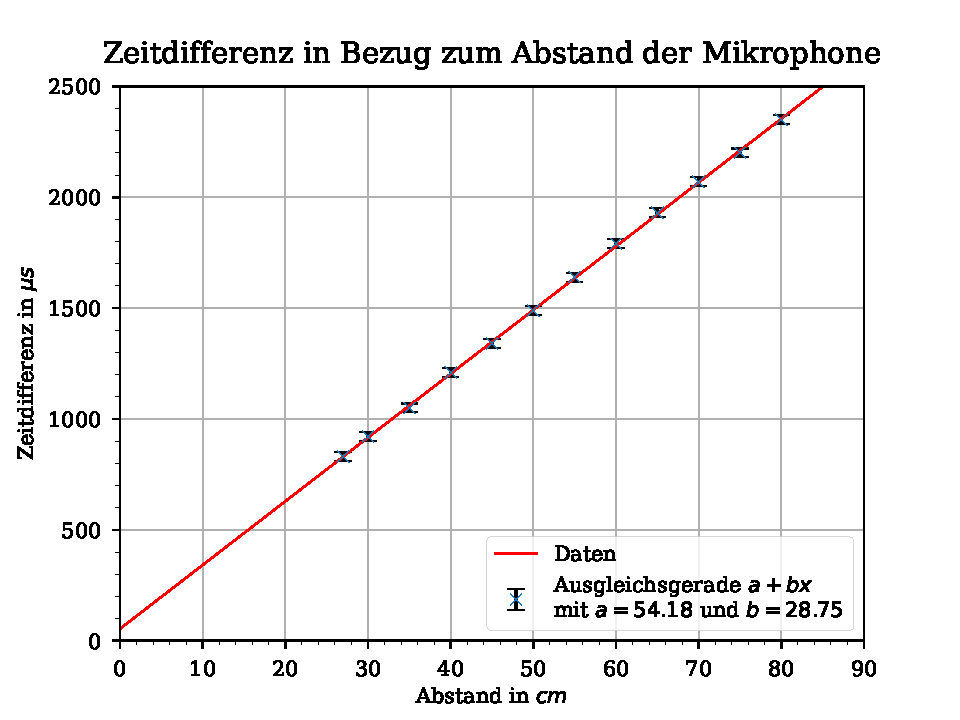
\includegraphics{./2Mikros.pdf}

        \caption{Meine Grafik}
        \label{fig:meine-grafik}
    \end{figure}


\end{document}